% Options for packages loaded elsewhere
\PassOptionsToPackage{unicode}{hyperref}
\PassOptionsToPackage{hyphens}{url}
\PassOptionsToPackage{dvipsnames,svgnames,x11names}{xcolor}
%
\documentclass[
  11pt,
  letterpaper,
  DIV=11,
  numbers=noendperiod]{scrartcl}

\usepackage{amsmath,amssymb}
\usepackage{iftex}
\ifPDFTeX
  \usepackage[T1]{fontenc}
  \usepackage[utf8]{inputenc}
  \usepackage{textcomp} % provide euro and other symbols
\else % if luatex or xetex
  \usepackage{unicode-math}
  \defaultfontfeatures{Scale=MatchLowercase}
  \defaultfontfeatures[\rmfamily]{Ligatures=TeX,Scale=1}
\fi
\usepackage{lmodern}
\ifPDFTeX\else  
    % xetex/luatex font selection
\fi
% Use upquote if available, for straight quotes in verbatim environments
\IfFileExists{upquote.sty}{\usepackage{upquote}}{}
\IfFileExists{microtype.sty}{% use microtype if available
  \usepackage[]{microtype}
  \UseMicrotypeSet[protrusion]{basicmath} % disable protrusion for tt fonts
}{}
\makeatletter
\@ifundefined{KOMAClassName}{% if non-KOMA class
  \IfFileExists{parskip.sty}{%
    \usepackage{parskip}
  }{% else
    \setlength{\parindent}{0pt}
    \setlength{\parskip}{6pt plus 2pt minus 1pt}}
}{% if KOMA class
  \KOMAoptions{parskip=half}}
\makeatother
\usepackage{xcolor}
\usepackage[margin=1in,heightrounded]{geometry}
\setlength{\emergencystretch}{3em} % prevent overfull lines
\setcounter{secnumdepth}{-\maxdimen} % remove section numbering
% Make \paragraph and \subparagraph free-standing
\ifx\paragraph\undefined\else
  \let\oldparagraph\paragraph
  \renewcommand{\paragraph}[1]{\oldparagraph{#1}\mbox{}}
\fi
\ifx\subparagraph\undefined\else
  \let\oldsubparagraph\subparagraph
  \renewcommand{\subparagraph}[1]{\oldsubparagraph{#1}\mbox{}}
\fi

\usepackage{color}
\usepackage{fancyvrb}
\newcommand{\VerbBar}{|}
\newcommand{\VERB}{\Verb[commandchars=\\\{\}]}
\DefineVerbatimEnvironment{Highlighting}{Verbatim}{commandchars=\\\{\}}
% Add ',fontsize=\small' for more characters per line
\newenvironment{Shaded}{}{}
\newcommand{\AlertTok}[1]{\textcolor[rgb]{0.16,0.16,0.16}{\textbf{\colorbox[rgb]{0.80,0.14,0.11}{#1}}}}
\newcommand{\AnnotationTok}[1]{\textcolor[rgb]{0.60,0.59,0.10}{#1}}
\newcommand{\AttributeTok}[1]{\textcolor[rgb]{0.84,0.60,0.13}{#1}}
\newcommand{\BaseNTok}[1]{\textcolor[rgb]{0.96,0.45,0.00}{#1}}
\newcommand{\BuiltInTok}[1]{\textcolor[rgb]{0.84,0.36,0.05}{#1}}
\newcommand{\CharTok}[1]{\textcolor[rgb]{0.69,0.38,0.53}{#1}}
\newcommand{\CommentTok}[1]{\textcolor[rgb]{0.57,0.51,0.45}{#1}}
\newcommand{\CommentVarTok}[1]{\textcolor[rgb]{0.57,0.51,0.45}{#1}}
\newcommand{\ConstantTok}[1]{\textcolor[rgb]{0.69,0.38,0.53}{\textbf{#1}}}
\newcommand{\ControlFlowTok}[1]{\textcolor[rgb]{0.80,0.14,0.11}{\textbf{#1}}}
\newcommand{\DataTypeTok}[1]{\textcolor[rgb]{0.84,0.60,0.13}{#1}}
\newcommand{\DecValTok}[1]{\textcolor[rgb]{0.96,0.45,0.00}{#1}}
\newcommand{\DocumentationTok}[1]{\textcolor[rgb]{0.60,0.59,0.10}{#1}}
\newcommand{\ErrorTok}[1]{\textcolor[rgb]{0.80,0.14,0.11}{\underline{#1}}}
\newcommand{\ExtensionTok}[1]{\textcolor[rgb]{0.41,0.62,0.42}{\textbf{#1}}}
\newcommand{\FloatTok}[1]{\textcolor[rgb]{0.96,0.45,0.00}{#1}}
\newcommand{\FunctionTok}[1]{\textcolor[rgb]{0.41,0.62,0.42}{#1}}
\newcommand{\ImportTok}[1]{\textcolor[rgb]{0.41,0.62,0.42}{#1}}
\newcommand{\InformationTok}[1]{\textcolor[rgb]{0.16,0.16,0.16}{\colorbox[rgb]{0.51,0.65,0.60}{#1}}}
\newcommand{\KeywordTok}[1]{\textcolor[rgb]{0.24,0.22,0.21}{\textbf{#1}}}
\newcommand{\NormalTok}[1]{\textcolor[rgb]{0.24,0.22,0.21}{#1}}
\newcommand{\OperatorTok}[1]{\textcolor[rgb]{0.24,0.22,0.21}{#1}}
\newcommand{\OtherTok}[1]{\textcolor[rgb]{0.41,0.62,0.42}{#1}}
\newcommand{\PreprocessorTok}[1]{\textcolor[rgb]{0.84,0.36,0.05}{#1}}
\newcommand{\RegionMarkerTok}[1]{\textcolor[rgb]{0.57,0.51,0.45}{\colorbox[rgb]{0.98,0.96,0.84}{#1}}}
\newcommand{\SpecialCharTok}[1]{\textcolor[rgb]{0.69,0.38,0.53}{#1}}
\newcommand{\SpecialStringTok}[1]{\textcolor[rgb]{0.60,0.59,0.10}{#1}}
\newcommand{\StringTok}[1]{\textcolor[rgb]{0.60,0.59,0.10}{#1}}
\newcommand{\VariableTok}[1]{\textcolor[rgb]{0.27,0.52,0.53}{#1}}
\newcommand{\VerbatimStringTok}[1]{\textcolor[rgb]{0.60,0.59,0.10}{#1}}
\newcommand{\WarningTok}[1]{\textcolor[rgb]{0.16,0.16,0.16}{\colorbox[rgb]{0.98,0.74,0.18}{#1}}}

\providecommand{\tightlist}{%
  \setlength{\itemsep}{0pt}\setlength{\parskip}{0pt}}\usepackage{longtable,booktabs,array}
\usepackage{calc} % for calculating minipage widths
% Correct order of tables after \paragraph or \subparagraph
\usepackage{etoolbox}
\makeatletter
\patchcmd\longtable{\par}{\if@noskipsec\mbox{}\fi\par}{}{}
\makeatother
% Allow footnotes in longtable head/foot
\IfFileExists{footnotehyper.sty}{\usepackage{footnotehyper}}{\usepackage{footnote}}
\makesavenoteenv{longtable}
\usepackage{graphicx}
\makeatletter
\def\maxwidth{\ifdim\Gin@nat@width>\linewidth\linewidth\else\Gin@nat@width\fi}
\def\maxheight{\ifdim\Gin@nat@height>\textheight\textheight\else\Gin@nat@height\fi}
\makeatother
% Scale images if necessary, so that they will not overflow the page
% margins by default, and it is still possible to overwrite the defaults
% using explicit options in \includegraphics[width, height, ...]{}
\setkeys{Gin}{width=\maxwidth,height=\maxheight,keepaspectratio}
% Set default figure placement to htbp
\makeatletter
\def\fps@figure{htbp}
\makeatother
\newlength{\cslhangindent}
\setlength{\cslhangindent}{1.5em}
\newlength{\csllabelwidth}
\setlength{\csllabelwidth}{3em}
\newlength{\cslentryspacingunit} % times entry-spacing
\setlength{\cslentryspacingunit}{\parskip}
\newenvironment{CSLReferences}[2] % #1 hanging-ident, #2 entry spacing
 {% don't indent paragraphs
  \setlength{\parindent}{0pt}
  % turn on hanging indent if param 1 is 1
  \ifodd #1
  \let\oldpar\par
  \def\par{\hangindent=\cslhangindent\oldpar}
  \fi
  % set entry spacing
  \setlength{\parskip}{#2\cslentryspacingunit}
 }%
 {}
\usepackage{calc}
\newcommand{\CSLBlock}[1]{#1\hfill\break}
\newcommand{\CSLLeftMargin}[1]{\parbox[t]{\csllabelwidth}{#1}}
\newcommand{\CSLRightInline}[1]{\parbox[t]{\linewidth - \csllabelwidth}{#1}\break}
\newcommand{\CSLIndent}[1]{\hspace{\cslhangindent}#1}

\KOMAoption{captions}{tableheading}
\makeatletter
\@ifpackageloaded{tcolorbox}{}{\usepackage[skins,breakable]{tcolorbox}}
\@ifpackageloaded{fontawesome5}{}{\usepackage{fontawesome5}}
\definecolor{quarto-callout-color}{HTML}{909090}
\definecolor{quarto-callout-note-color}{HTML}{0758E5}
\definecolor{quarto-callout-important-color}{HTML}{CC1914}
\definecolor{quarto-callout-warning-color}{HTML}{EB9113}
\definecolor{quarto-callout-tip-color}{HTML}{00A047}
\definecolor{quarto-callout-caution-color}{HTML}{FC5300}
\definecolor{quarto-callout-color-frame}{HTML}{acacac}
\definecolor{quarto-callout-note-color-frame}{HTML}{4582ec}
\definecolor{quarto-callout-important-color-frame}{HTML}{d9534f}
\definecolor{quarto-callout-warning-color-frame}{HTML}{f0ad4e}
\definecolor{quarto-callout-tip-color-frame}{HTML}{02b875}
\definecolor{quarto-callout-caution-color-frame}{HTML}{fd7e14}
\makeatother
\makeatletter
\makeatother
\makeatletter
\makeatother
\makeatletter
\@ifpackageloaded{caption}{}{\usepackage{caption}}
\AtBeginDocument{%
\ifdefined\contentsname
  \renewcommand*\contentsname{Table of contents}
\else
  \newcommand\contentsname{Table of contents}
\fi
\ifdefined\listfigurename
  \renewcommand*\listfigurename{List of Figures}
\else
  \newcommand\listfigurename{List of Figures}
\fi
\ifdefined\listtablename
  \renewcommand*\listtablename{List of Tables}
\else
  \newcommand\listtablename{List of Tables}
\fi
\ifdefined\figurename
  \renewcommand*\figurename{Figure}
\else
  \newcommand\figurename{Figure}
\fi
\ifdefined\tablename
  \renewcommand*\tablename{Table}
\else
  \newcommand\tablename{Table}
\fi
}
\@ifpackageloaded{float}{}{\usepackage{float}}
\floatstyle{ruled}
\@ifundefined{c@chapter}{\newfloat{codelisting}{h}{lop}}{\newfloat{codelisting}{h}{lop}[chapter]}
\floatname{codelisting}{Listing}
\newcommand*\listoflistings{\listof{codelisting}{List of Listings}}
\makeatother
\makeatletter
\@ifpackageloaded{caption}{}{\usepackage{caption}}
\@ifpackageloaded{subcaption}{}{\usepackage{subcaption}}
\makeatother
\makeatletter
\makeatother
\ifLuaTeX
  \usepackage{selnolig}  % disable illegal ligatures
\fi
\IfFileExists{bookmark.sty}{\usepackage{bookmark}}{\usepackage{hyperref}}
\IfFileExists{xurl.sty}{\usepackage{xurl}}{} % add URL line breaks if available
\urlstyle{same} % disable monospaced font for URLs
\hypersetup{
  pdftitle={Problem Set \#1},
  pdfauthor={Salvador Balkus},
  colorlinks=true,
  linkcolor={blue},
  filecolor={Maroon},
  citecolor={Blue},
  urlcolor={Blue},
  pdfcreator={LaTeX via pandoc}}

\title{Problem Set \#1}
\usepackage{etoolbox}
\makeatletter
\providecommand{\subtitle}[1]{% add subtitle to \maketitle
  \apptocmd{\@title}{\par {\large #1 \par}}{}{}
}
\makeatother
\subtitle{BST 258: Causal Inference -- Theory and Practice}
\author{Salvador Balkus}
\date{}

\begin{document}
\maketitle
\hypertarget{question-1}{%
\subsection{Question 1}\label{question-1}}

Insert link to github repo

\hypertarget{question-2}{%
\subsection{Question 2}\label{question-2}}

\hypertarget{a}{%
\subsubsection{(a)}\label{a}}

\begin{tcolorbox}[enhanced jigsaw, breakable, leftrule=.75mm, toprule=.15mm, arc=.35mm, bottomrule=.15mm, left=2mm, opacityback=0, colback=white, colframe=quarto-callout-note-color-frame, rightrule=.15mm]

\textbf{Answer}\vspace{2mm}

Assuming \(A_i \in \{0, 1\}\), the marginal distribution of the first
sampled unit \(i\) is \(P(A_i = 1) = \frac{m}{n}\) and
\(P(A_i = 0) = 1 - \frac{m}{n} = \frac{n - m}{n}\).

\end{tcolorbox}

\hypertarget{b}{%
\subsubsection{(b)}\label{b}}

\begin{tcolorbox}[enhanced jigsaw, breakable, leftrule=.75mm, toprule=.15mm, arc=.35mm, bottomrule=.15mm, left=2mm, opacityback=0, colback=white, colframe=quarto-callout-note-color-frame, rightrule=.15mm]

\textbf{Answer}\vspace{2mm}

WLOG, assume that \(A_i\)'s treatment is sampled first, then \(A_j\).
Then,

\(P(A_i = a_i, A_j = a_j) = P(A_j = a_j | A_i = a_i) \cdot P(A_i = a_i)\)

Plugging in part (a) and noting that the number of total units and
treated units for \(A_j\) is reduced by 1 after sampling \(A_i\), we
find that the joint distribution of \(A_i\) and \(A_j\) is given by:

\begin{itemize}
\tightlist
\item
  \(P(A_i = 1, A_j = 1) = \frac{m}{n} \cdot \frac{m-1}{n-1} = \frac{m(m-1)}{n(n-1)}\)
\item
  \(P(A_i = 0, A_j = 1) = \frac{m}{n} \cdot \Big(1 - \frac{m-1}{n-1}\Big) = \frac{m(n-m)}{n(n-1)}\)
\item
  \(P(A_i = 1, A_j = 0) = \Big(1 - \frac{m}{n}\Big) \cdot \Big(\frac{m}{n-1}\Big) = \frac{m(n-m)}{n(n-1)}\)
\item
  \(P(A_i = 0, A_j = 0) = \Big(1 - \frac{m}{n}\Big) \cdot \Big(1 - \frac{m-1}{n-1}\Big) = \frac{(n-m)^2}{n(n-1)}\)
\end{itemize}

Then the joint pmf is given by the following table:

~~~~~~~~~~\textbar{} \(A_i = 0\) \textbar{} \(A_i = 1\) \textbar{}\\
\(A_j = 0\) \textbar{} \(\frac{(n-m)^2}{n(n-1)}\) \textbar{}
\(\frac{m(n-m)}{n(n-1)}\) \textbar{}\\
\(A_j = 1\) \textbar{} \(\frac{m(n-m)}{n(n-1)}\) \textbar{}
\(\frac{m(m-1)}{n(n-1)}\) \textbar{}

\end{tcolorbox}

\hypertarget{c}{%
\subsubsection{(c)}\label{c}}

\textbf{Variance}: Since \(A_i\) is marginally
\(\text{Bernoulli}(\frac{m}{n})\), the variance is known to be

\(\mathbb{V}(A_i) = \frac{m}{n}(1 - \frac{m}{n}) = \frac{m}{n}(\frac{n - m}{n})\).

Note that \(E(A_i) = P(A_i = 1) = \frac{m}{n}\); then, one can derive
this as

\(\mathbb{V}(A_i) = E(A_i^2) - E(A_i)^2 = \sum_{a_i = 0}^1 a_i^2\cdot P(A_i = a_i) - (\frac{m}{n})^2 = \frac{m}{n}(1 - \frac{m}{n}\)

which gives the same result.

\textbf{Covariance}: Using the property of covariance that
\(Cov(A_i, A_j) = E(A_iA_j) - E(A_i)E(A_j)\), we can first note that
\(E(A_i) = E(A_j) = P(A_i = 1) = \frac{m}{n}\). Additionally,
\(E(A_iA_j) = P(A_i = 1, A_j = 1) = \frac{m(m-1)}{n(n-1)}\) from the
joint probability table solved in part (b). Therefore, the covariance is

\(Cov(A_i, A_j) = \frac{m(m-1)}{n(n-1)} - \frac{m^2}{n^2} = frac{nm^2 - nm - m^2n + m^2}{n^2(n-1)} = -\frac{1}{n}(\frac{m(n-m)}{n(n-1)})\)

\hypertarget{d}{%
\subsubsection{(d)}\label{d}}

We can compute the expectation of the sample ATT using the linearity of
expectation, noting that \(A_i \perp\!\!\!\!\perp Y_i(a)\) by definition
of a CRE, and that \(E(A_i) = P(A_i = 1) = \frac{m}{n}\). Therefore, we
have

\begin{Shaded}
\begin{Highlighting}[]
\NormalTok{\textbackslash{}begin\{align*\}}
\NormalTok{E(\textbackslash{}theta\^{}\{ATT\}) = \textbackslash{}frac\{1\}\{m\}\textbackslash{}sum\_\{i=1\}\^{}nE(A\_i(Y\_i(1) {-} Y\_i(0)))\textbackslash{}\textbackslash{}}
\NormalTok{= \textbackslash{}frac\{n\}\{m\} E(A\_i) E(Y\_i(1) {-} Y\_i(0))\textbackslash{}\textbackslash{}}
\NormalTok{= \textbackslash{}frac\{n\}\{m\} \textbackslash{}frac\{m\}\{n\} E(Y\_i(1) {-} Y\_i(0))}
\NormalTok{= E(Y\_i(1) {-} Y\_i(0)) = \textbackslash{}theta\^{}\{ATE\}}
\NormalTok{\textbackslash{}end\{align*\}}
\end{Highlighting}
\end{Shaded}

So, in expectation, the sample ATT is equal to the population ATE (that
is, \(E(\theta^{ATT}) = \theta^{ATE}\)).

\newpage{}

\hypertarget{question-3}{%
\subsection{Question 3}\label{question-3}}

:::\{.callout-note title=``Answer''\}

Since \(Y_i(1) = Y_i(0) + \theta\), we have the property of variance
that \(\mathbb{V}(X + b) = \mathbb{V}(X)\). Even when considering the
sample variance, this follows because

\(\mathbb{V}(X + b) = \mathbb{E}((X + b - \mathbb{E}(X + b))^2) = \mathbb{E}((X - \mathbb{E}(X))^2) = \mathbb{V}(X)\)

with \(b\) canceling due to linearity of expectation. Therefore,
substituting in the given equality we have

\(\mathbb{V}(Y_i(1)) = \mathbb{V}(Y_i(0) + \theta) = \mathbb{V}(Y_i(0))\)

Using this, we can note the similar property of covariance that
\(Cov(X + b, Y + c) = Cov(X, Y)\); in the sample setting this follows
from

\(Cov(X + b, Y + c) = \mathbb{E}((X + b - \mathbb{E}(X + b))(X + c - \mathbb{E}(X + c))) = \mathbb{E}((X - \mathbb{E}(X))(X - \mathbb{E}(X)))= Cov(X, Y)\)

Using this property, we have that

\begin{Shaded}
\begin{Highlighting}[]
\NormalTok{\textbackslash{}begin\{align*\}}
\NormalTok{\textbackslash{}rho(Y\_i(1), Y\_i(0)) = \textbackslash{}frac\{Cov(Y\_i(1), Y\_i(0))\}\{\textbackslash{}sqrt\{\textbackslash{}mathbb\{V\}(Y\_i(1))\textbackslash{}cdot\textbackslash{}mathbb\{V\}(Y\_i(0))\}\}\textbackslash{}\textbackslash{}}
\NormalTok{= \textbackslash{}frac\{Cov(Y\_i(0) + \textbackslash{}theta, Y\_i(0))\}\{\textbackslash{}sqrt\{\textbackslash{}mathbb\{V\}(Y\_i(0))\textbackslash{}cdot \textbackslash{}mathbb\{V\}(Y\_i(0))\}\}\textbackslash{}\textbackslash{}}
\NormalTok{= \textbackslash{}frac\{Cov(Y\_i(0), Y\_i(0))\}\{\textbackslash{}sqrt\{\textbackslash{}mathbb\{V\}(Y\_i(0))\^{}2\}\}= \textbackslash{}frac\{\textbackslash{}mathbb\{V\}(Y\_i(0))\}\{\textbackslash{}mathbb\{V\}(Y\_i(0))\} = 1\textbackslash{}\textbackslash{}}
\NormalTok{\textbackslash{}end\{align*\}}
\end{Highlighting}
\end{Shaded}

thereby completing the proof. \(\square\)

::

\newpage{}

\hypertarget{question-4}{%
\subsection{Question 4}\label{question-4}}

\begin{tcolorbox}[enhanced jigsaw, breakable, leftrule=.75mm, toprule=.15mm, arc=.35mm, bottomrule=.15mm, left=2mm, opacityback=0, colback=white, colframe=quarto-callout-note-color-frame, rightrule=.15mm]

\textbf{Answer}\vspace{2mm}

There are 70 possible ways to choose 4 out of 8 cups as those that had
tea poured first (thereby leaving the remaining 4 as those that had milk
poured first). This is because
\({8 \choose 4} = \frac{8!}{4!(8-4)!} = 70\).

Therefore, the probability of guessing \(k\) cups correctly is
\({4 \choose k} \cdot {4 \choose 4-k} \cdot \frac{1}{70}\). That is, the
probability is the product the number of possible ways to choose \(k\)
cups correctly and the number of possible ways to choose the remaining
\(4-k\) cups incorrectly, divided by the total number of possible ways
to choose 4 cups.

Hence, we have:

\begin{itemize}
\tightlist
\item
  Probability of 0 cups correct: \(\frac{1}{70}\) (only one possibility,
  all four wrong)
\item
  Probability of 1 cup correct:
  \({4\choose 3} \cdot {4\choose 1} \cdot \frac{1}{70} = \frac{16}{70}\)
\item
  Probability of 2 cups correct:
  \({4\choose 2} \cdot {4\choose 2} \cdot \frac{1}{70} = \frac{36}{70}\)
\item
  Probability of 3 cups correct:
  \({4\choose 1} \cdot {4\choose 3} \cdot \frac{1}{70} = \frac{16}{70}\)
\item
  Probability of 4 cups correct: \(\frac{1}{70}\) (only one possibility,
  all four correct)
\end{itemize}

\end{tcolorbox}

\newpage{}

\hypertarget{question-5}{%
\subsection{Question 5}\label{question-5}}

\hypertarget{a-1}{%
\subsubsection{(a)}\label{a-1}}

\begin{tcolorbox}[enhanced jigsaw, breakable, leftrule=.75mm, toprule=.15mm, arc=.35mm, bottomrule=.15mm, left=2mm, opacityback=0, colback=white, colframe=quarto-callout-note-color-frame, rightrule=.15mm]

\textbf{Answer}\vspace{2mm}

\emph{First}, we can notice that those with large kidney stones received
Treatment A much more often (263/343 times, \textasciitilde77\%), while
those with small kidney stones received Treatment B more often (234/357
times, \textasciitilde66\%). \emph{Second}, we can also note that those
who experienced large stones had a lower probability of being
successfully treated across both treatments (73\% large versus 93\%
small for A, 69\% large versus 87\% small for B).

Putting these two facts together, we can conclude that Treatment B
probably appeared more successful in aggregate because it was more
frequently used to treat small kidney stones, the type of outcome more
likely to be treated succesfully regardless of treatment type. However,
in reality, if we ``control'' for outcome type via stratification,
Treatment A is actually more effective -- which is probably why it was
more frequently used for cases of large kidney stones that were ``more
difficult'' to treat.

\end{tcolorbox}

\hypertarget{b-1}{%
\subsubsection{(b)}\label{b-1}}

\begin{tcolorbox}[enhanced jigsaw, breakable, leftrule=.75mm, toprule=.15mm, arc=.35mm, bottomrule=.15mm, left=2mm, opacityback=0, colback=white, colframe=quarto-callout-note-color-frame, rightrule=.15mm]

\textbf{Answer}\vspace{2mm}

~~~~~~~~~~~~~~\textbar{} Treatment A \textbar{} Treatment B \textbar{}\\
Male, Small \textbar{} 95\% (74/78) \textbar{} 99\% (69/70) \textbar{}\\
Female, Small \textbar{} 77\% (7/9) \textbar{} 83\% (165/200)
\textbar{}\\
Male, Large \textbar{} 49\% (21/43) \textbar{} 62\% (37/60) \textbar{}\\
Female, Large \textbar{} 78\% (171/220) \textbar{} 90\% (18/20)
\textbar{}\\
All \textbar{} 78\% (273/350) \textbar{} 83\% (289/350) \textbar{}

\end{tcolorbox}

\hypertarget{c-1}{%
\subsubsection{(c)}\label{c-1}}

\begin{tcolorbox}[enhanced jigsaw, breakable, leftrule=.75mm, toprule=.15mm, arc=.35mm, bottomrule=.15mm, left=2mm, opacityback=0, colback=white, colframe=quarto-callout-note-color-frame, rightrule=.15mm]

\textbf{Answer}\vspace{2mm}

This phenomenon is known as \textbf{Simpson's Paradox} (Pearl
(\protect\hyperlink{ref-Pearl2014}{2014})): when the association between
two varaibles reverses upon conditioning of a third variable. For causal
inference, it implies that in order to obtain a true causal
relationship, we need to control for confounding variables that might
change the probability of a given treatment assignment. Otherwise, a
situation might arise in which one treatment appears better only because
it was more likely to be assigned to an individual more likely to
exhibit a positive outcome -- not because it is more effective.

\end{tcolorbox}

\newpage{}

\hypertarget{question-6}{%
\subsection{Question 6}\label{question-6}}

\begin{Shaded}
\begin{Highlighting}[]
\ImportTok{using} \BuiltInTok{Distributions}
\ImportTok{using} \BuiltInTok{Plots}
\ImportTok{using} \BuiltInTok{Random}

\KeywordTok{function} \FunctionTok{run\_trial}\NormalTok{(μ₀, μ₁, σ², n, α, n\_sim, B)}

  \CommentTok{\# sample counterfactuals}
\NormalTok{  Y1 }\OperatorTok{=} \FunctionTok{rand}\NormalTok{(}\FunctionTok{Normal}\NormalTok{(μ₁, }\FunctionTok{sqrt}\NormalTok{(σ²)), n)}
\NormalTok{  Y0 }\OperatorTok{=} \FunctionTok{rand}\NormalTok{(}\FunctionTok{Normal}\NormalTok{(μ₀, }\FunctionTok{sqrt}\NormalTok{(σ²)), n)}

  \CommentTok{\# sample treatment assignment matrix}
\NormalTok{  A }\OperatorTok{=} \FunctionTok{rand}\NormalTok{(}\FunctionTok{Bernoulli}\NormalTok{(}\FloatTok{0.5}\NormalTok{), n, n\_sim)}
\NormalTok{  Y }\OperatorTok{=} \FunctionTok{map}\NormalTok{(A }\OperatorTok{{-}\textgreater{}}\NormalTok{ (@. A }\OperatorTok{*}\NormalTok{ Y1 }\OperatorTok{+}\NormalTok{ (}\FloatTok{1} \OperatorTok{{-}}\NormalTok{ A) }\OperatorTok{*}\NormalTok{ Y0), }\FunctionTok{eachcol}\NormalTok{(A))}

  \CommentTok{\# calculate difference{-}in{-}means test statistic across simulations}
  \FunctionTok{m1}\NormalTok{(Y, A) }\OperatorTok{=} \FunctionTok{mean}\NormalTok{(Y[A }\OperatorTok{.==} \FloatTok{1}\NormalTok{]) }
  \FunctionTok{m0}\NormalTok{(Y, A) }\OperatorTok{=} \FunctionTok{mean}\NormalTok{(Y[A }\OperatorTok{.==} \FloatTok{0}\NormalTok{])}
  \FunctionTok{dif\_in\_means}\NormalTok{(Y, A) }\OperatorTok{=} \FunctionTok{abs}\NormalTok{(}\FunctionTok{m1}\NormalTok{(Y, A) }\OperatorTok{{-}} \FunctionTok{m0}\NormalTok{(Y, A))}
\NormalTok{  ψ\_ate }\OperatorTok{=}\NormalTok{ [}\FunctionTok{dif\_in\_means}\NormalTok{(Y[i], A[}\OperatorTok{:}\NormalTok{, i]) for i }\KeywordTok{in} \FloatTok{1}\OperatorTok{:}\NormalTok{n\_sim]}

  \CommentTok{\# calculate sharp null p{-}values}
  \FunctionTok{sharp\_null}\NormalTok{(Y, A, ψ) }\OperatorTok{=} \FunctionTok{mean}\NormalTok{(}\FunctionTok{dif\_in\_means}\NormalTok{(Y, }\FunctionTok{shuffle}\NormalTok{(A)) }\OperatorTok{\textgreater{}=}\NormalTok{ ψ }\ControlFlowTok{for}\NormalTok{ \_ }\KeywordTok{in} \FloatTok{1}\OperatorTok{:}\NormalTok{B)}
\NormalTok{  p\_sharp }\OperatorTok{=}\NormalTok{ [}\FunctionTok{sharp\_null}\NormalTok{(Y[i], A[}\OperatorTok{:}\NormalTok{, i], ψ\_ate[i]) for i }\KeywordTok{in} \FloatTok{1}\OperatorTok{:}\NormalTok{n\_sim]}

  \CommentTok{\# calculate weak null p{-}values}
\NormalTok{  p\_est }\OperatorTok{=} \FunctionTok{mean}\NormalTok{(A, dims }\OperatorTok{=} \FloatTok{1}\NormalTok{)}
  \FunctionTok{var\_ate}\NormalTok{(Y, A, p) }\OperatorTok{=}\NormalTok{ (}\FunctionTok{var}\NormalTok{(Y[A }\OperatorTok{.==} \FloatTok{1}\NormalTok{]) }\OperatorTok{/}\NormalTok{ p) }\OperatorTok{+}\NormalTok{ (}\FunctionTok{var}\NormalTok{(Y[A }\OperatorTok{.==} \FloatTok{0}\NormalTok{]) }\OperatorTok{/}\NormalTok{ (}\FloatTok{1} \OperatorTok{{-}}\NormalTok{ p))}
\NormalTok{  σ²\_est }\OperatorTok{=}\NormalTok{ [}\FunctionTok{var\_ate}\NormalTok{(Y[i], A[}\OperatorTok{:}\NormalTok{, i], p\_est[i]) for i }\KeywordTok{in} \FloatTok{1}\OperatorTok{:}\NormalTok{n\_sim]}
\NormalTok{  p\_weak }\OperatorTok{=}\NormalTok{ @. }\FloatTok{2}\FunctionTok{*}\NormalTok{(}\FloatTok{1} \OperatorTok{{-}} \FunctionTok{cdf}\NormalTok{(}\FunctionTok{Normal}\NormalTok{(}\FloatTok{0}\NormalTok{, }\FunctionTok{sqrt}\NormalTok{(σ²\_est }\OperatorTok{/}\NormalTok{ n)), ψ\_ate))}

  \CommentTok{\# calculate power of the trial}
\NormalTok{  power\_sharp }\OperatorTok{=} \FunctionTok{mean}\NormalTok{(p\_sharp }\OperatorTok{.\textless{}}\NormalTok{ α)}
\NormalTok{  power\_weak }\OperatorTok{=} \FunctionTok{mean}\NormalTok{(p\_weak }\OperatorTok{.\textless{}}\NormalTok{ α)}

  \ControlFlowTok{return}\NormalTok{ power\_sharp, power\_weak}
\ControlFlowTok{end}
\end{Highlighting}
\end{Shaded}

\begin{verbatim}
run_trial (generic function with 1 method)
\end{verbatim}

\begin{Shaded}
\begin{Highlighting}[]
\BuiltInTok{Random}\NormalTok{.}\FunctionTok{seed!}\NormalTok{(}\FloatTok{1}\NormalTok{)}
\NormalTok{ns }\OperatorTok{=}\NormalTok{ [}\FloatTok{20}\NormalTok{, }\FloatTok{50}\NormalTok{, }\FloatTok{100}\NormalTok{, }\FloatTok{200}\NormalTok{, }\FloatTok{500}\NormalTok{]}
\NormalTok{μ₀ }\OperatorTok{=} \FloatTok{0}
\NormalTok{μ₁ }\OperatorTok{=} \FloatTok{1}\OperatorTok{/}\FloatTok{10}
\NormalTok{σ² }\OperatorTok{=} \FloatTok{1}\OperatorTok{/}\FloatTok{16}
\NormalTok{α }\OperatorTok{=} \FloatTok{0.05}
\NormalTok{n\_sim }\OperatorTok{=} \FloatTok{1000}
\NormalTok{B }\OperatorTok{=} \FloatTok{10000}

\NormalTok{result }\OperatorTok{=}\NormalTok{ [}\FunctionTok{run\_trial}\NormalTok{(μ₀, μ₁, σ², n, α, n\_sim, B) for n }\KeywordTok{in}\NormalTok{ ns]}
\NormalTok{power\_sharp }\OperatorTok{=}\NormalTok{ [r[}\FloatTok{1}\NormalTok{] for r }\KeywordTok{in}\NormalTok{ result]}
\NormalTok{power\_weak }\OperatorTok{=}\NormalTok{ [r[}\FloatTok{2}\NormalTok{] for r }\KeywordTok{in}\NormalTok{ result]}
\end{Highlighting}
\end{Shaded}

\begin{verbatim}
5-element Vector{Float64}:
 0.037
 0.086
 0.34
 0.991
 1.0
\end{verbatim}

\begin{Shaded}
\begin{Highlighting}[]
\FunctionTok{plot}\NormalTok{([power\_sharp, power\_weak], }
\NormalTok{          marker }\OperatorTok{=} \OperatorTok{:}\NormalTok{circle,}
\NormalTok{          xticks }\OperatorTok{=}\NormalTok{ (}\FloatTok{1}\OperatorTok{:}\FloatTok{5}\NormalTok{, }\FunctionTok{string}\NormalTok{.(ns)),}
\NormalTok{          xaxis }\OperatorTok{=} \StringTok{"Samples"}\NormalTok{, }
\NormalTok{          yaxis }\OperatorTok{=} \StringTok{"Power"}\NormalTok{,}
\NormalTok{          labels }\OperatorTok{=}\NormalTok{ [}\StringTok{"Sharp Null"} \StringTok{"Weak Null"}\NormalTok{])}
\end{Highlighting}
\end{Shaded}

\begin{figure}[H]

{\centering 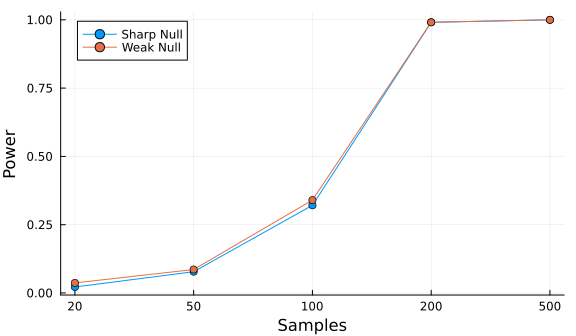
\includegraphics{PS1_files/mediabag/PS1_files/figure-pdf/cell-5-output-1.pdf}

}

\end{figure}

\newpage{}

\hypertarget{question-7}{%
\subsection{Question 7}\label{question-7}}

\hypertarget{a-2}{%
\subsubsection{(a)}\label{a-2}}

We can solve the linear program

\(\min_{\alpha,\beta} \frac{1}{2n} \sum_{i=1}^n(Y_i - \alpha - \beta A_i)^2\)

using the first derivative test, setting the partial derivatives to 0 to
obtain solutions:

\begin{Shaded}
\begin{Highlighting}[]
\NormalTok{\textbackslash{}begin\{align*\}}
\NormalTok{  \textbackslash{}frac\{\textbackslash{}partial\}\{\textbackslash{}partial \textbackslash{}alpha\} L(\textbackslash{}alpha, \textbackslash{}beta) = {-}\textbackslash{}frac\{1\}\{n\} \textbackslash{}sum\_\{i=1\}\^{}n(Y\_i {-} \textbackslash{}alpha {-} \textbackslash{}beta A\_i) = 0\textbackslash{}\textbackslash{}}
\NormalTok{  \textbackslash{}implies \textbackslash{}hat\{\textbackslash{}alpha\} =  \textbackslash{}beta \textbackslash{}bar\{A\} {-} \textbackslash{}bar\{Y\}}
\NormalTok{\textbackslash{}end\{align*\}}
\end{Highlighting}
\end{Shaded}

and

\begin{Shaded}
\begin{Highlighting}[]
\NormalTok{\textbackslash{}begin\{align*\}}
\NormalTok{  \textbackslash{}frac\{\textbackslash{}partial\}\{\textbackslash{}partial \textbackslash{}beta\} L(\textbackslash{}alpha, \textbackslash{}beta) = {-}\textbackslash{}frac\{1\}\{n\} \textbackslash{}sum\_\{i=1\}\^{}n(Y\_i {-} \textbackslash{}alpha {-} \textbackslash{}beta A\_i)A\_i = 0\textbackslash{}\textbackslash{}}
\NormalTok{  \textbackslash{}implies \textbackslash{}hat\{\textbackslash{}beta\} = \textbackslash{}frac\{\textbackslash{}alpha \textbackslash{}bar\{A\} {-} \textbackslash{}frac\{1\}\{n\}\textbackslash{}sum\_\{i=1\}\^{}nA\_iY\_i\}\{\textbackslash{}bar\{A\^{}2\}\}}
\NormalTok{\textbackslash{}end\{align*\}}
\end{Highlighting}
\end{Shaded}

Plugging in the solution for \(\alpha\) into the solution for \(\beta\),
we obtain

\begin{Shaded}
\begin{Highlighting}[]
\NormalTok{\textbackslash{}begin\{align*\}}
\NormalTok{\textbackslash{}beta = \textbackslash{}frac\{\textbackslash{}beta(\textbackslash{}bar\{A\})\^{}2 {-} \textbackslash{}bar\{A\}\textbackslash{}bar\{Y\} {-} \textbackslash{}frac\{1\}\{n\}\textbackslash{}sum\_\{i=1\}\^{}nA\_iY\_i\}\{\textbackslash{}bar\{A\^{}2\}\}\textbackslash{}\textbackslash{}}
\NormalTok{\textbackslash{}implies \textbackslash{}beta(\textbackslash{}frac\{\textbackslash{}bar\{A\}\^{}2 {-} \textbackslash{}bar\{A\^{}2\}\}\{\textbackslash{}cancel\{\textbackslash{}bar\{A\^{}2\}\}\}) = \textbackslash{}frac\{\textbackslash{}bar\{A\}\textbackslash{}bar\{Y\} {-} \textbackslash{}frac\{1\}\{n\}\textbackslash{}sum\_\{i=1\}\^{}nA\_iY\_i\}\{\textbackslash{}cancel\{\textbackslash{}bar\{A\^{}2\}\}\}\textbackslash{}\textbackslash{}}
\NormalTok{\textbackslash{}implies \textbackslash{}hat\{\textbackslash{}beta\} = \textbackslash{}frac\{\textbackslash{}sum(Y\_i {-} \textbackslash{}bar\{Y\})(A\_i {-} \textbackslash{}bar\{A\}\}\{\textbackslash{}sum(A\_i {-} \textbackslash{}bar\{A\})\^{}2\}}
\NormalTok{\textbackslash{}end\{align*\}}
\end{Highlighting}
\end{Shaded}

and therefore

\begin{Shaded}
\begin{Highlighting}[]
\NormalTok{\textbackslash{}hat\{\textbackslash{}alpha\} =  \textbackslash{}hat\{\textbackslash{}beta\}\textbackslash{}bar\{A\} {-} \textbackslash{}bar\{Y\} = \textbackslash{}hat\{\textbackslash{}beta\} = \textbackslash{}frac\{\textbackslash{}sum(Y\_i {-} \textbackslash{}bar\{Y\})(A\_i {-} \textbackslash{}bar\{A\}\}\{\textbackslash{}sum(A\_i {-} \textbackslash{}bar\{A\})\^{}2\}\textbackslash{}bar\{A\} {-} \textbackslash{}bar\{Y\}}
\end{Highlighting}
\end{Shaded}

By the second derivative test, we can take the partial derivatives to
get

\begin{Shaded}
\begin{Highlighting}[]
\NormalTok{\textbackslash{}begin\{align*\}}
\NormalTok{\textbackslash{}frac\{\textbackslash{}partial\}\{\textbackslash{}partial \textbackslash{}alpha\^{}2\} L(\textbackslash{}alpha, \textbackslash{}beta) = n\textbackslash{}\textbackslash{}}
\NormalTok{\textbackslash{}frac\{\textbackslash{}partial\}\{\textbackslash{}partial \textbackslash{}beta\^{}2\} L(\textbackslash{}alpha, \textbackslash{}beta) = \textbackslash{}frac\{1\}\{n\}\textbackslash{}sum\_\{i=1\}\^{}nA\_i\^{}2\textbackslash{}\textbackslash{}}
\NormalTok{\textbackslash{}frac\{\textbackslash{}partial\}\{\textbackslash{}partial \textbackslash{}alpha\textbackslash{}partial \textbackslash{}beta\} L(\textbackslash{}alpha, \textbackslash{}beta) = \textbackslash{}bar\{A\}}
\NormalTok{\textbackslash{}end\{align*\}}
\end{Highlighting}
\end{Shaded}

Now, since \(A \in \{0, 1\}\), we have

\begin{Shaded}
\begin{Highlighting}[]
\NormalTok{\textbackslash{}begin\{align*\}}
\NormalTok{D(\textbackslash{}alpha, \textbackslash{}beta) = n\textbackslash{}cdot \textbackslash{}frac\{1\}\{n\}\textbackslash{}sum\_\{i=1\}\^{}nA\_i\^{}2 {-} \textbackslash{}bar\{A\} = \textbackslash{}\textbackslash{}}
\NormalTok{\textbackslash{}sum\_\{i=1\}\^{}nA\_i {-} \textbackslash{}frac\{1\}\{n\}\textbackslash{}sum\_\{i=1\}\^{}nA\_i = \textbackslash{}frac\{n{-}1\}\{n\} \textgreater{} 0}
\NormalTok{\textbackslash{}end\{align*\}}
\end{Highlighting}
\end{Shaded}

and by the second derivative test, \(D(\alpha, \beta) > 0\) and
\(\frac{\partial}{\partial \alpha^2} L(\alpha, \beta) = n > 0\) implies
\((\hat{\alpha}, \hat{\beta})\) is a minimum. It must be a global
minimum since it was found to be a unique critical point in the first
derivative test, therefore the endpoints cannot be smaller.

Therefore, the solution to the linear program is

\(\hat{\beta} = \frac{\sum(Y_i - \bar{Y})(A_i - \bar{A}}{\sum(A_i - \bar{A})^2}\)

and

\(\hat{\alpha} = \frac{\sum(Y_i - \bar{Y})(A_i - \bar{A}}{\sum(A_i - \bar{A})^2}\bar{A} - \bar{Y}\)

\hypertarget{b-2}{%
\subsubsection{(b)}\label{b-2}}

Yes, \$\hat{\beta} is a valid estimator of the ATE. We can show this by
proving it is unbiased; that \(E(\hat{\beta}) = \beta)\). Note that by
construction of the completely randomized experiment,
\(\bar{A} = \frac{m}{n}\). Therefore,

\begin{Shaded}
\begin{Highlighting}[]
\NormalTok{\textbackslash{}begin\{align*\}}
\NormalTok{\textbackslash{}sum\_\{i=1\}\^{}n (A\_i {-} \textbackslash{}bar\{A\})\^{}2 = sum\_\{i=1\}\^{}nA\_i\^{}2 {-} 2\textbackslash{}frac\{m\}\{n\}sum\_\{i=1\}\^{}nA{-}i + sum\_\{i=1\}\^{}n(\textbackslash{}frac\{m\}\{n\})\^{}2\textbackslash{}\textbackslash{}}
\NormalTok{= m {-} 2m + \textbackslash{}frac\{m\^{}2\}\{n\} = \textbackslash{}frac\{m(m{-}n)\}\{n\}}
\NormalTok{\textbackslash{}end\{align*\}}
\end{Highlighting}
\end{Shaded}

Therefore, it is a constant that can be moved outside the expectation.

Then, noting that the numerator of \(\hat{\beta}\) is
\((\hat{Y})(\hat{A}) - \frac{1}{n}\sum_{i=1}^n A_i Y_i\) from part (a),
we can substitute \(Y_i = A_i Y_i(1) + (1 - A_i) Y_i(0)\) and use
linearity of expectation to evaluate the left and right terms of the
subtraction separately.

The expectation of the first term in the subtraction reduces to

\begin{Shaded}
\begin{Highlighting}[]
\NormalTok{\textbackslash{}begin\{align*\}}
\NormalTok{E(\textbackslash{}bar\{A\}\textbackslash{}bar\{Y\}) = \textbackslash{}frac\{m\}\{n\}E(A\_iY\_i(1) + (1{-}A\_i)Y\_i(0))\textbackslash{}\textbackslash{}}
\NormalTok{= \textbackslash{}frac\{m\^{}2\}\{n\} E(Y\_i(1)) + \textbackslash{}frac\{m(n{-}m)\}\{n\}E(Y\_i(0))}
\NormalTok{\textbackslash{}end\{align*\}}
\end{Highlighting}
\end{Shaded}

The expectation of the second term in the subtraction reduces to

\begin{Shaded}
\begin{Highlighting}[]
\NormalTok{\textbackslash{}begin\{align*\}}
\NormalTok{E(\textbackslash{}frac\{1\}\{n\}\textbackslash{}sum\_\{i=1\}\^{}n A\_i Y\_i) = E(A\_i\^{}2Y\_i(1) + A\_i(1 {-} A\_i)Y\_i(1)) = \textbackslash{}frac\{m\}\{n\}E(Y\_i(1))}
\NormalTok{\textbackslash{}end\{align*\}}
\end{Highlighting}
\end{Shaded}

Now, combining these terms and dividing by the denominator
\(\frac{m(m-n)}{n}\) solved previously, we have

\begin{Shaded}
\begin{Highlighting}[]
\NormalTok{\textbackslash{}begin\{align*\}}
\NormalTok{E(\textbackslash{}hat\{\textbackslash{}beta\}) = (m(\textbackslash{}frac\{m{-}n\}\{n\})E(Y\_i(1)) {-} \textbackslash{}frac\{m(m{-}n)\}\{n\}E(Y\_i(0)) {-}  \textbackslash{}frac\{m\}\{n\}E(Y\_i(1))) / \textbackslash{}frac\{m(m{-}n)\}\{n\}\textbackslash{}\textbackslash{}}
\NormalTok{= (m(\textbackslash{}frac\{m{-}n\}\{n\})E(Y\_i(1)) {-} \textbackslash{}frac\{m(m{-}n)\}\{n\}E(Y\_i(0))) / \textbackslash{}frac\{m(m{-}n)\}\{n\} \textbackslash{}\textbackslash{}}
\NormalTok{= E(Y\_i(0)) {-} E(Y\_i(1))}
\end{Highlighting}
\end{Shaded}

which is the definition of the ATE. Therefore,
\(E(\hat{\beta}) = E(Y_i(0) - Y_i(1))\) meaning it is an unbiased, and
therefore valid estimator of the ATE.

\hypertarget{acknowledgements}{%
\section{Acknowledgements}\label{acknowledgements}}

A disclosure for academic honesty: GitHub Copilot was used to prepare
this assignment. However, only minor uses of the text/code autocomplete
feature were used.

\hypertarget{references}{%
\subsection{References}\label{references}}

\hypertarget{refs}{}
\begin{CSLReferences}{1}{0}
\leavevmode\vadjust pre{\hypertarget{ref-Pearl2014}{}}%
Pearl, Judea. 2014. {``Comment: Understanding Simpson's Paradox.''}
\emph{The American Statistician} 68 (1): 8--13.
\url{https://doi.org/10.1080/00031305.2014.876829}.

\end{CSLReferences}



\end{document}
